\documentclass[a4paper,12 pt]{article}
\usepackage{geometry}
\geometry{letterpaper, margin=0.8in}
\usepackage[english]{babel}
\usepackage[utf8]{inputenc}
\usepackage{enumitem}
\setlist{  
  listparindent=\parindent,
  parsep=0pt,
}
\usepackage{amsmath}
\usepackage{graphicx}
\usepackage[colorinlistoftodos]{todonotes}
\usepackage{float}
\usepackage{amssymb}
\usepackage{bbm}
\usepackage[normalem]{ulem}
\usepackage{natbib}
\usepackage{listings}


\title{\vspace{-2.0cm}CSCI 6360: Parallel Computing Assignment 2 Report}
\author{Anirban Das (dasa2@rpi.edu) }
\date{February 20, 2018}


\begin{document}
\maketitle

\textbf{All execution times include the time taken for the whole program to complete, this includes the time taken to read the file, which in my case was not a bottleneck as the ripple carry adder took around 0.056 seconds to run including file reading.}
\begin{enumerate}
\item \textbf{Plot of the execution time of 2, 4, 8 and 16 rank runs as function of their number of ranks}:\\
\begin{figure}[H]
	\centering
	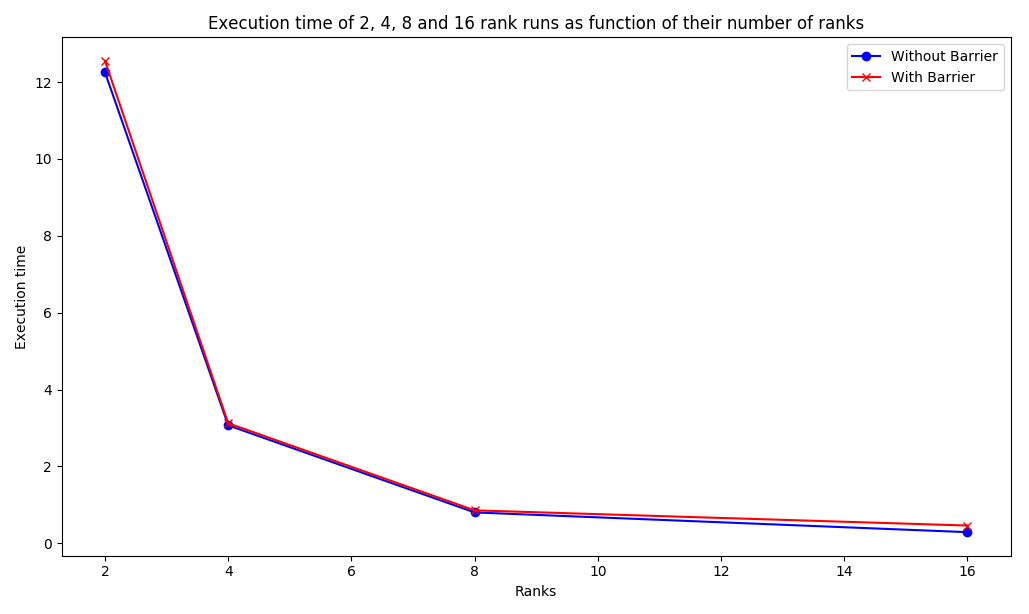
\includegraphics[width=.8\linewidth]{Graphs/graph_1.png}
  \caption{Execution time versus Number of ranks = 2, 4, 8, 16}
\end{figure}
We can easily see that the execution time goes down with increasing parallelism i.e. with increasing number of ranks. In case of more than one ranks, the execution time used is the average execution time obtained from all ranks. The following is a chart of the average runtimes obtained:
\begin{table}[]
\centering
\caption{Runtime of different Rank MPI CLA runs with/ without Barriers}
\label{my-label}
\begin{tabular}{|l|c|l|c|l|l|}
\hline
Ranks                       & 1 (Serial)                   & 2       & 4                           & 8      & 16     \\ \hline
Runtime With Barrier (s)    & 48.5256                      & 12.5498 & 3.1244                      & 0.8593 & 0.4643 \\ \hline
Runtime Without Barrier (s) & \multicolumn{1}{l|}{48.1984} & 12.2502 & \multicolumn{1}{l|}{3.0720} & 0.8054 & 0.2920 \\ \hline
\end{tabular}
\end{table}

Also , it is noted that the execution time is always greater when barrier is used (line in red), that simple case without barrier (line in blue). This can be explained by the fact that since using MPI\_Barrier essentially synchronises all the ranks, by keeping them in step with one another, hence the average run time is dictated by the straggler rank or the one with the largest execution time. Hence with barrier, we usually see slightly larger execution time.

The following is the same graph, but with a semi log Y axis, so that the difference between barrier and without barrier lines are more prominent:
\begin{figure}[H]
	\centering
	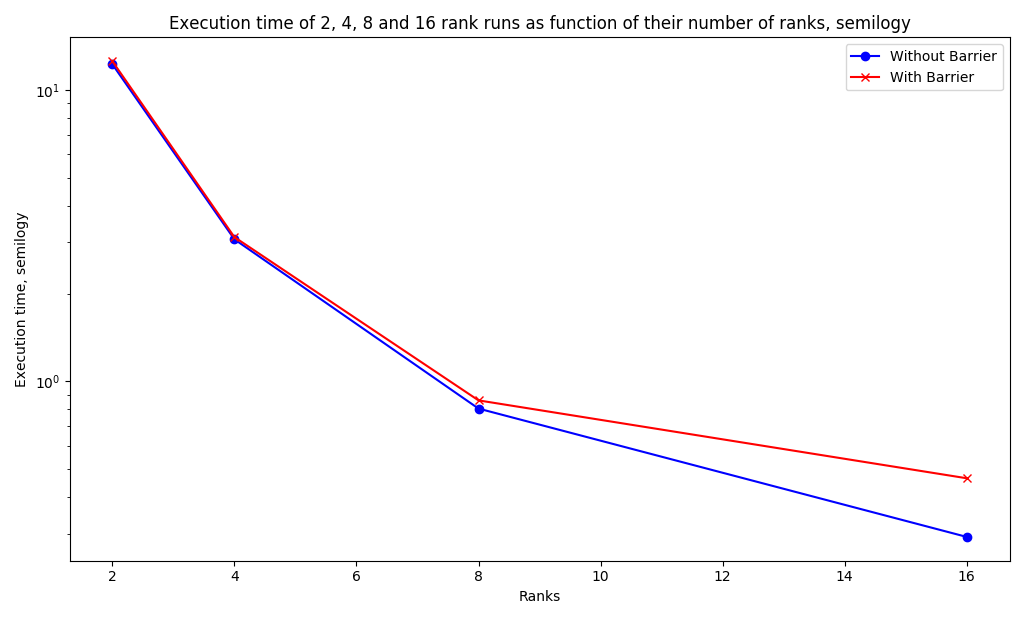
\includegraphics[width=.8\linewidth]{Graphs/graph_1_semilogy.png}
  \caption{Execution time versus Number of ranks = 2, 4, 8, 16 (Y axis in semilog)}
\end{figure}

\item \textbf{Plot of speedup relative to the execution time o serial MPI CLA added to 2, 4, 8 and 16 rank runs}:\\

The following is the plot of the speed up of 2, 4, 8, 16 rank MPI CLA runs w.r.t. MPI CLA run with rank 1, i.e. serial MPI CLA execution. The times of speedup is on the y axis and in in $log_{10}$ scale to produce an appropiately scaled graph.

\begin{figure}[H]
	\centering
	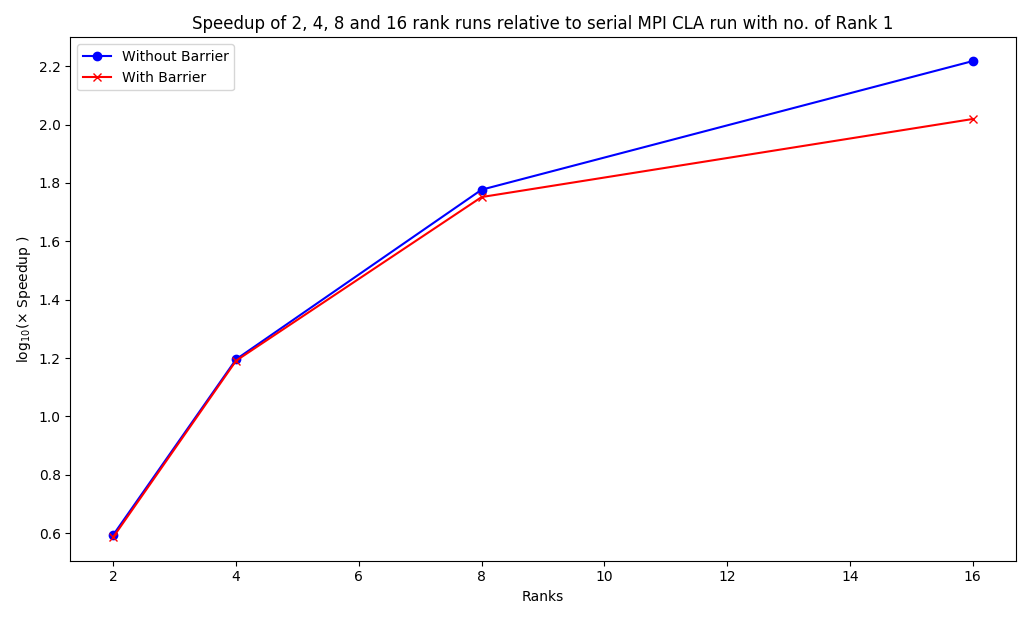
\includegraphics[width=.8\linewidth]{Graphs/graph_2.png}
  \caption{$\log_{10}(\times $Speedup) w.r.t. 1 Rank MPI CLA run vs Number of Ranks}
\end{figure}

We can see that with barrier, the speed up is not as much as without barrier. This is because of the same reason as mentioned in the previous graph. 

Also it is observed that with increase in number of Ranks used, the speed up increases. This is because of the fact that with increasing Ranks, the calculation is broken down in smaller units and processed parallely, whereas in serial run, the whole computation is done in a single node. Therefor we can see upto a $10^{2.2} \times$ speedup in 16 Ranks w.r.t. serial MPI run, or in other words, the serial MPI CLA execution is $10^{2.2}$ larger than what we obtained in 16 Ranks MPI Cla run.

Serial MPI CLA runs with and without barrier were around 48.1984s and 48.5256s respectively, whereas the average runtime of for e.g. 16 Ranks, with and without barrier are 0.4643s and 0.2920s respectively. 


\item \textbf{Plot the speedup of the relative to the execution time of the serial ripple carry adder
to the MPI CLA adder running in parallel on 2 through 16 ranks}:\\

The CLA ripple carry adder is insanely fast, computing the result in about \textbf{0.0566 seconds}. It is pure C code, there is no MPI message passing, initializing etc overheads. Hence compared to it we will see 'negative' speedups. That is the speed of execution of all MPI CLA runs from 2 to 16 Ranks will be higher in comparison to the ripple carry adder. The following is the graph with $\frac{\text{Execution time of Ripple Carry Adder}}{\text{Execution time of Ith Rank MPI CLA execution}}$ on the Y axis with the number of ranks of the X axis:

\begin{figure}[H]
	\centering
	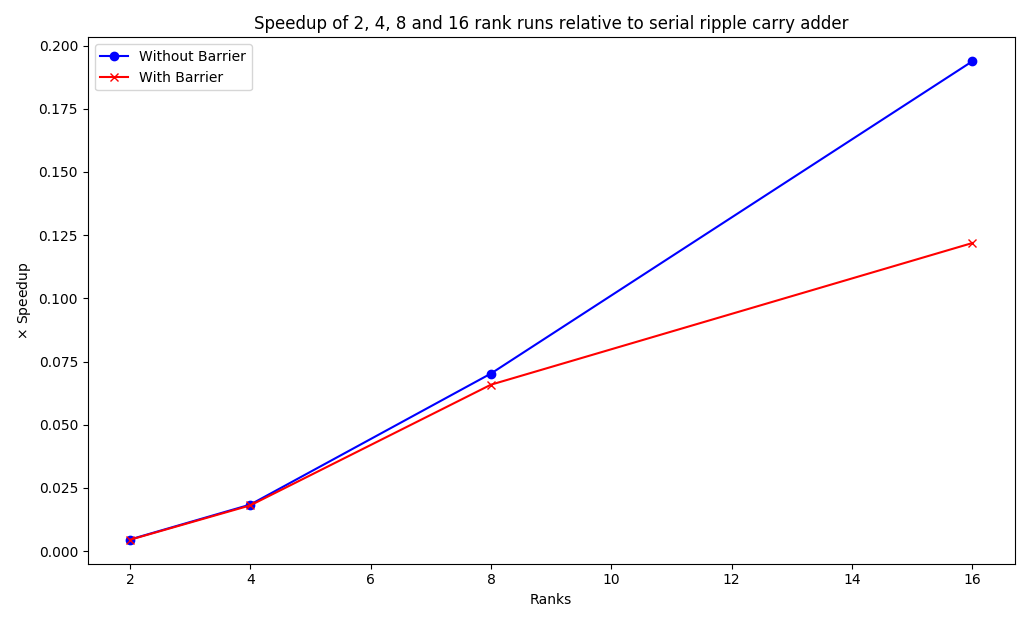
\includegraphics[width=.8\linewidth]{Graphs/graph_3.png}
  \caption{$(\times $Speedup) w.r.t. Ripple Carry Adder run vs Number of Ranks}
\end{figure}

As usual , we see the same behaviour. The execution time of 16 RANK MPI CLA execution is however the closest to the ripple carry adder timing, giving a mere $0.2\times$ speedup without barrier and $0.122 \times$ speedup with barrier w.r.t. to ripple carry adder. The lowest speedup is obtained when we compare 2 Rank MPI CLA run with the ripple carry adder : $\frac{0.0566}{12.25} = 0.0046$ without barrier and $\frac{0.0566}{12.5498} = 0.0045$ with barrier respectively.


\end{enumerate}



\end{document}